In the “Sub-Groups” section of this chapter, we described collective functions and how collective functions express common communication patterns. We specifically discussed the broadcast collective function, which is used to communicate a value from one work-item in a group to the other work-items in the group. This section describes additional collective functions.\par

Although the collective functions described in this section can be implemented directly in our programs using features such as atomics, work-group local memory, and barriers, many devices include dedicated hardware to accelerate collective functions. Even when a device does not include specialized hardware, vendor-provided implementations of collective functions are likely tuned for the device they are running on, so calling a built-in collective function will usually perform better than a general-purpose implementation that we might write.\par

\begin{tcolorbox}[colback=red!5!white,colframe=red!75!black]
Use collective functions for common communication patterns to simplify code and increase performance!
\end{tcolorbox}

Many collective functions are supported for both work-groups and sub-groups. Other collective functions are supported only for sub-groups\par

\hspace*{\fill} \par %插入空行
\textbf{Broadcast}

The broadcast function enables one work-item in a group to share the value of a variable with all other work-items in the group. A diagram showing how the broadcast function works can be found in Figure 9-12. The broadcast function is supported for both work-groups and subgroups.\par

\hspace*{\fill} \par %插入空行
\textbf{Votes}

The any\_of and all\_of functions (henceforth referred to collectively as “vote” functions) enable work-items to compare the result of a Boolean condition across their group: any\_of returns true if the condition is true for at least one work-item in the group, and all\_of returns true only if the condition is true for all work-items in the group. A comparison of these two functions for an example input is shown in Figure 9-15.\par

\hspace*{\fill} \par %插入空行
Figure 9-15. Comparison of the any\_of and all\_of functions
\begin{center}
	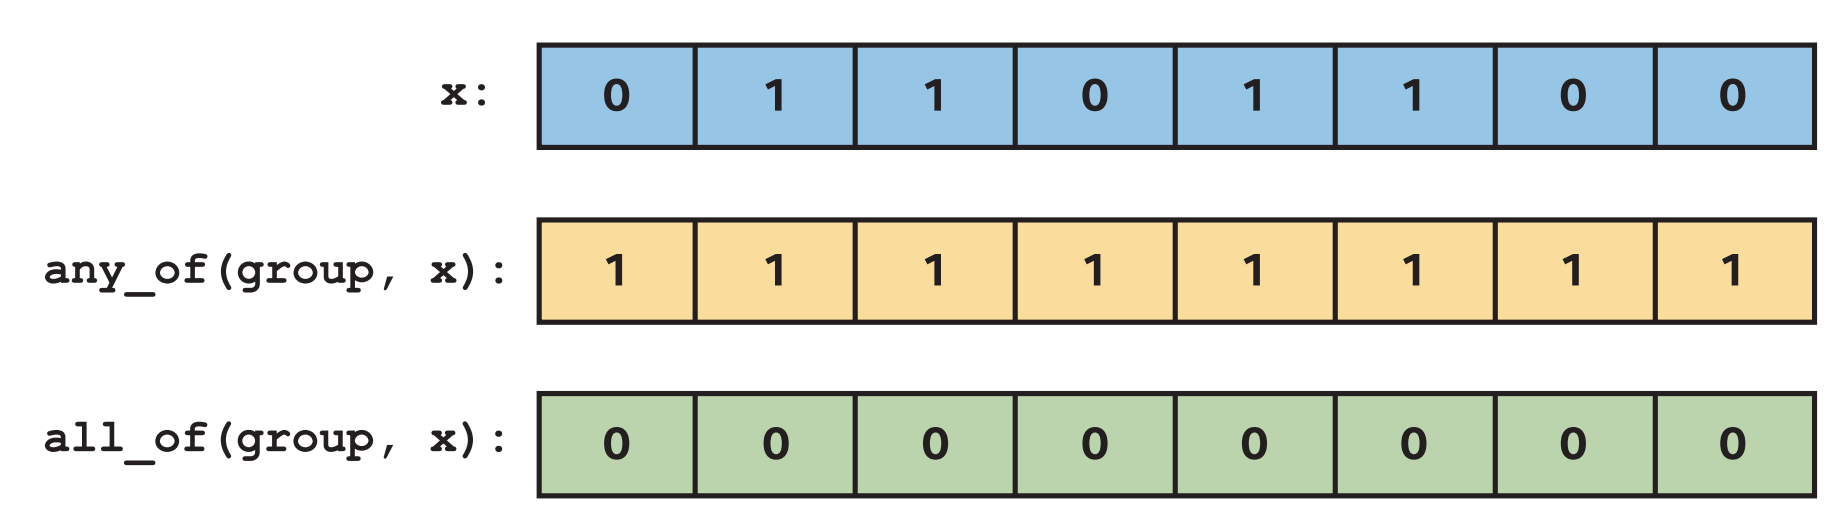
\includegraphics[width=1.\textwidth]{content/chapter-9/images/8}
\end{center}

The any\_of and all\_of vote functions are supported for both workgroups and sub-groups.\par

\hspace*{\fill} \par %插入空行
\textbf{Shuffles}

One of the most useful features of sub-groups is the ability to communicate directly between individual work-items without explicit memory operations. In many cases, such as the sub-group matrix multiplication kernel, these shuffle operations enable us to remove work-group local memory usage from our kernels and/or to avoid unnecessary repeated accesses to global memory. There are several flavors of these shuffle functions available.\par

The most general of the shuffle functions is called shuffle, and as shown in Figure 9-16, it allows for arbitrary communication between any pair of work-items in the sub-group. This generality may come at a performance cost, however, and we strongly encourage making use of the more specialized shuffle functions wherever possible.\par

In Figure 9-16, a generic shuffle is used to sort the x values of a subgroup using pre-computed permutation indices. Arrows are shown for one work-item in the sub-group, where the result of the shuffle is the value of x for the work-item with local\_id equal to 7.\par

\hspace*{\fill} \par %插入空行
Figure 9-16. Using a generic shuffle to sort x values based on precomputed permutation indices
\begin{center}
	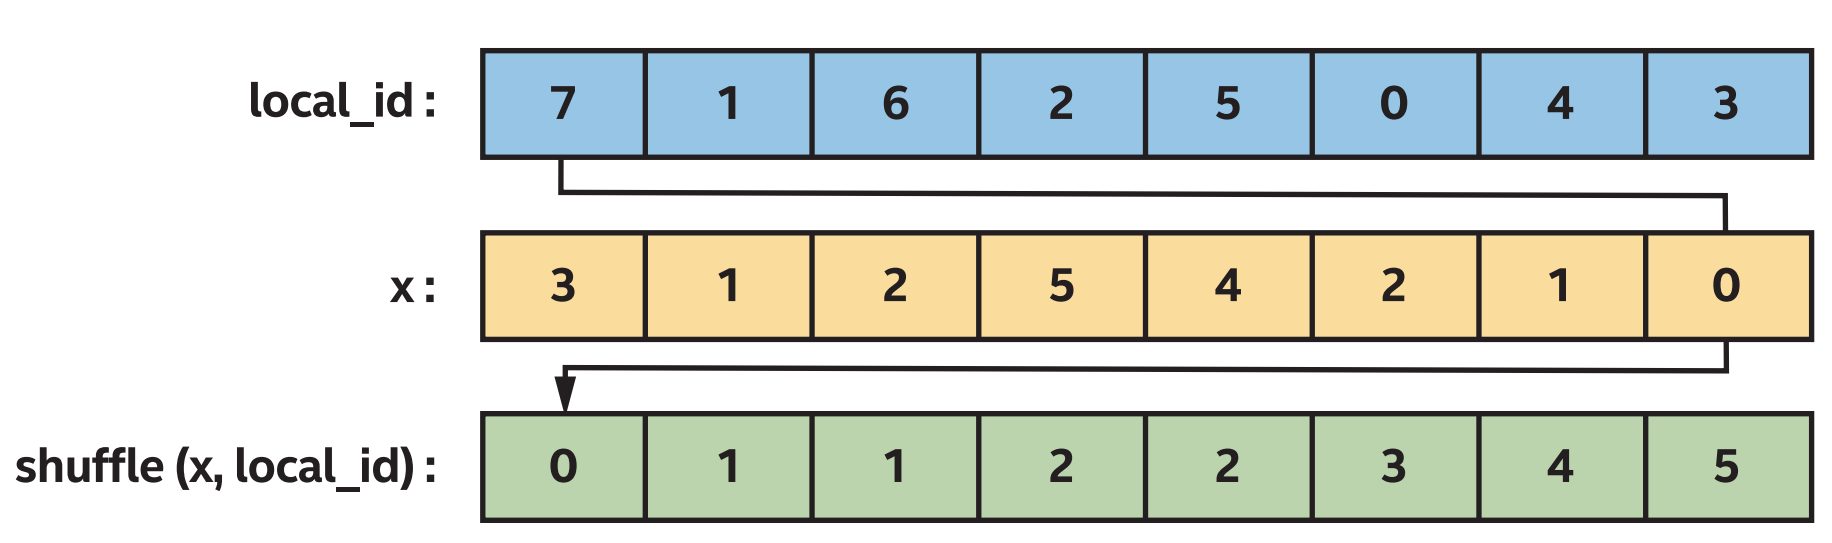
\includegraphics[width=1.\textwidth]{content/chapter-9/images/9}
\end{center}

Note that the sub-group broadcast function can be thought of as a specialized version of the general-purpose shuffle function, where the shuffle index is the same for all work-items in the sub-group. When the shuffle index is known to be the same for all work-items in the sub-group, using broadcast instead of shuffle provides the compiler additional information and may increase performance on some implementations.\par

The shuffle\_up and shuffle\_down functions effectively shift the contents of a sub-group by a fixed number of elements in a given direction, as shown in Figure 9-17. Note that the values returned to the last five work-items in the sub-group are undefined and are shown as blank in Figure 9-17. Shifting can be useful for parallelizing loops with loopcarried dependences or when implementing common algorithms such as exclusive or inclusive scans.\par

\hspace*{\fill} \par %插入空行
Figure 9-17. Using shuffle\_down to shift x values of a sub-group by five items
\begin{center}
	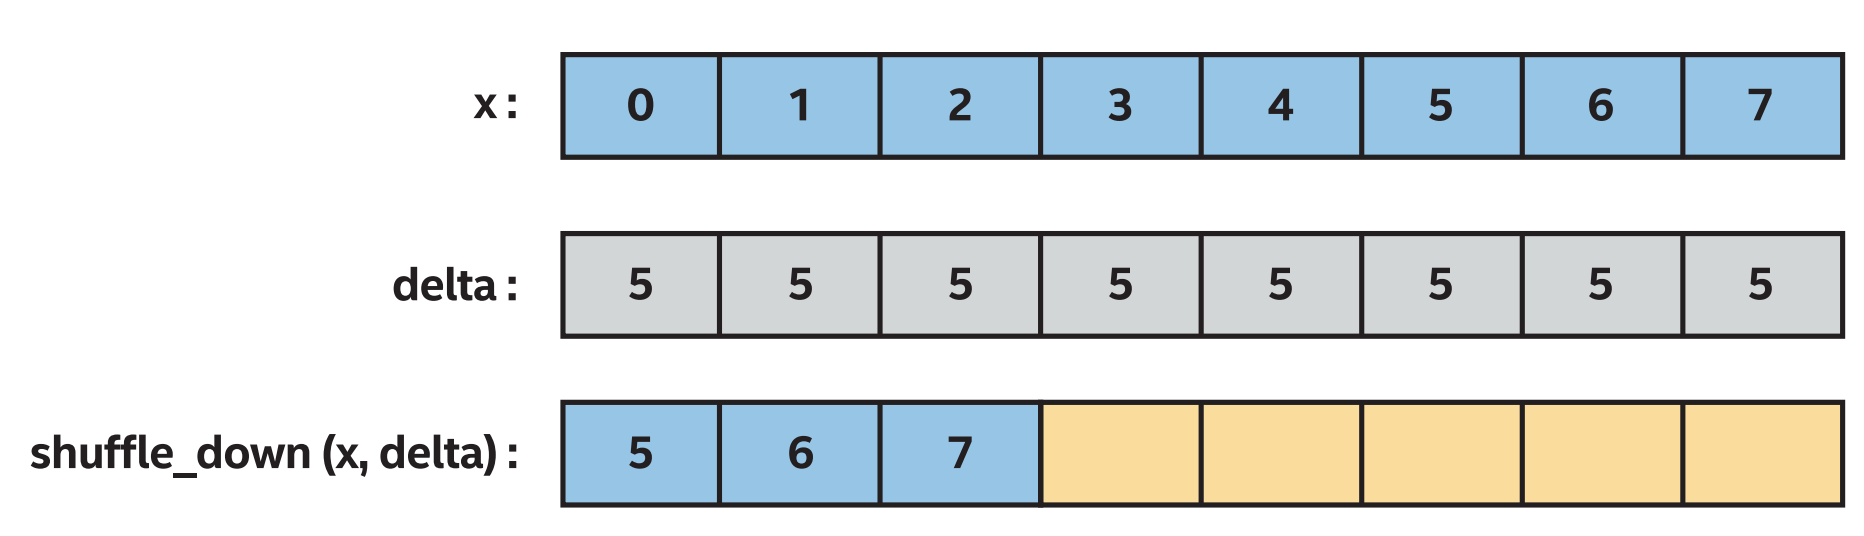
\includegraphics[width=1.\textwidth]{content/chapter-9/images/10}
\end{center}

The shuffle\_xor function swaps the values of two work-items, as specified by the result of an XOR operation applied to the work-item's sub-group local id and a fixed constant. As shown in Figures 9-18 and 9-19, several common communication patterns can be expressed using an XOR: for example, swapping pairs of neighboring values.\par

\hspace*{\fill} \par %插入空行
Figure 9-18. Swapping neighboring pairs of x using a shuffle\_xor
\begin{center}
	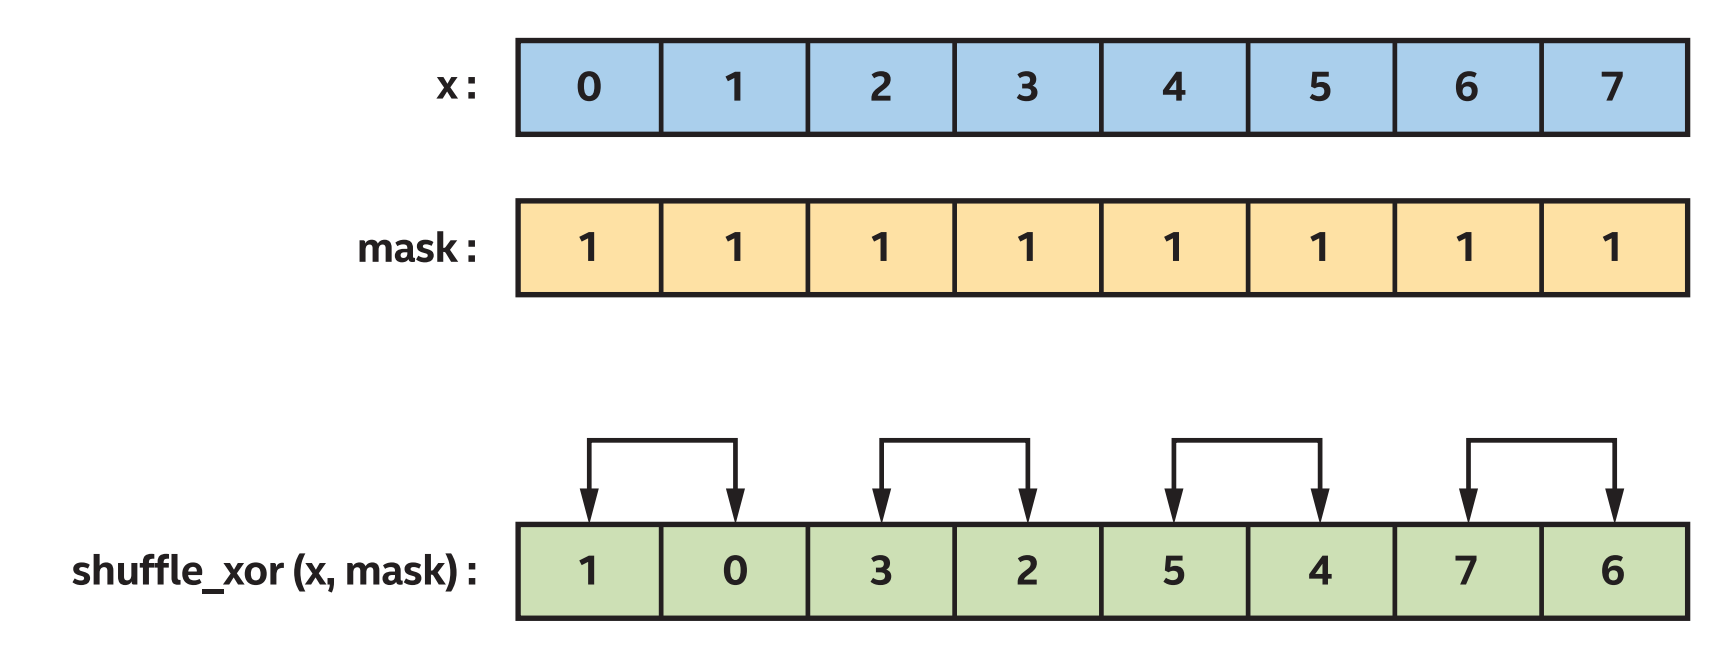
\includegraphics[width=1.\textwidth]{content/chapter-9/images/11}
\end{center}

or reversing the sub-group values.\par

\hspace*{\fill} \par %插入空行
Figure 9-19. Reverse the values of x using a shuffle\_xor
\begin{center}
	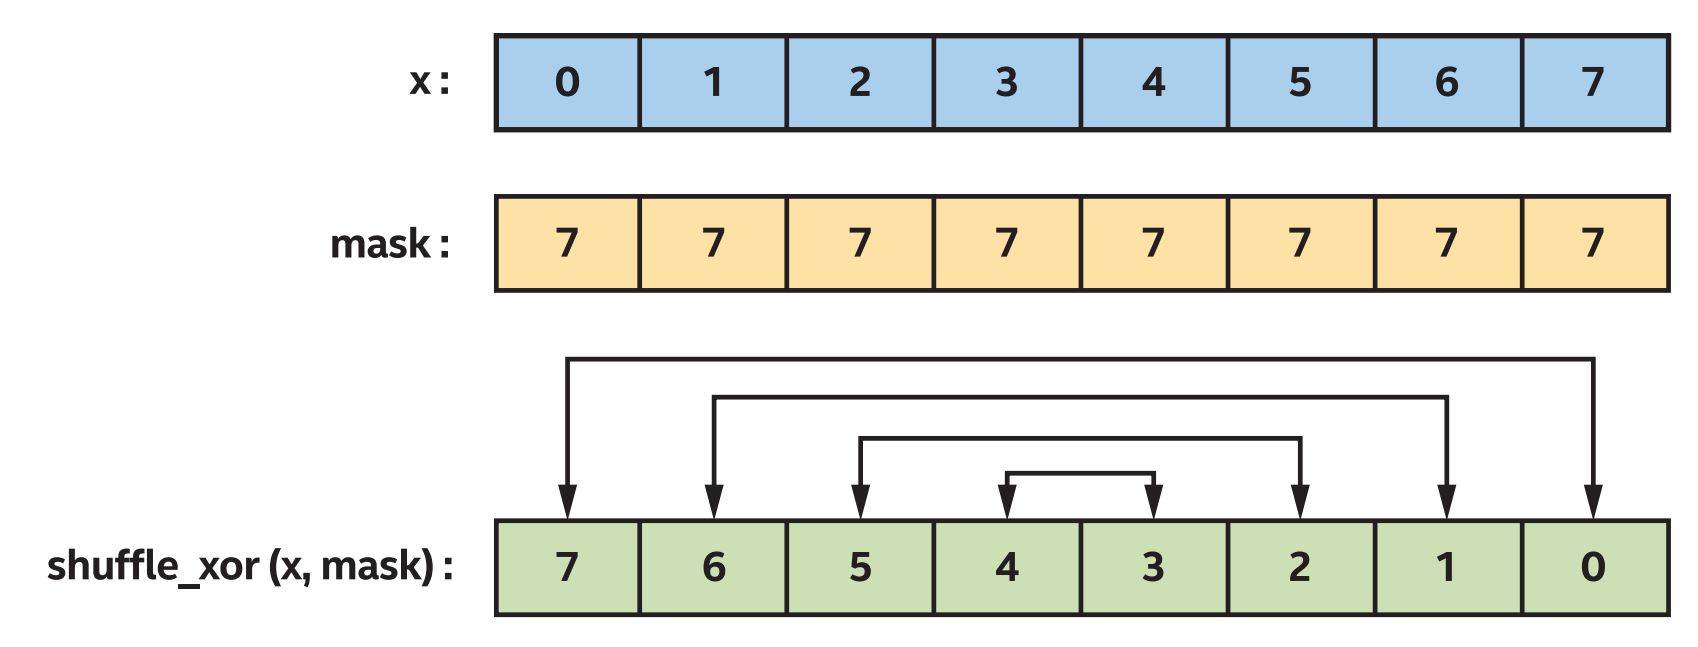
\includegraphics[width=1.\textwidth]{content/chapter-9/images/12}
\end{center}

\begin{tcolorbox}[colback=blue!5!white,colframe=blue!75!black, title=SUB-GROUP OPTIMIZATIONS USING BROADCAST VOTE AND COLLECTIVES]
The behavior of broadcast, vote, and other collective functions applied to subgroups is identical to when they are applied to work-groups, but they deserve additional attention because they may enable aggressive optimizations in certain compilers. For example, a compiler may be able to reduce register usage for variables that are broadcast to all work-items in a sub-group or may be able to reason about control flow divergence based on usage of the any\_of and all\_of functions.
\end{tcolorbox}

\hspace*{\fill} \par %插入空行
\textbf{Loads and Stores}

The sub-group load and store functions serve two purposes: first, informing the compiler that all work-items in the sub-group are loading contiguous data starting from the same (uniform) location in memory and, second, enabling us to request optimized loads/stores of large amounts of contiguous data.\par

For an ND-range parallel\_for, it may not be clear to the compiler how addresses computed by different work-items relate to one another. For example, as shown in Figure 9-20, accessing a contiguous block of memory from indices [0, 32) appears to have a strided access pattern from the perspective of each work-item.\par

\hspace*{\fill} \par %插入空行
Figure 9-20. Memory access pattern of a sub-group accessing four contiguous blocks
\begin{center}
	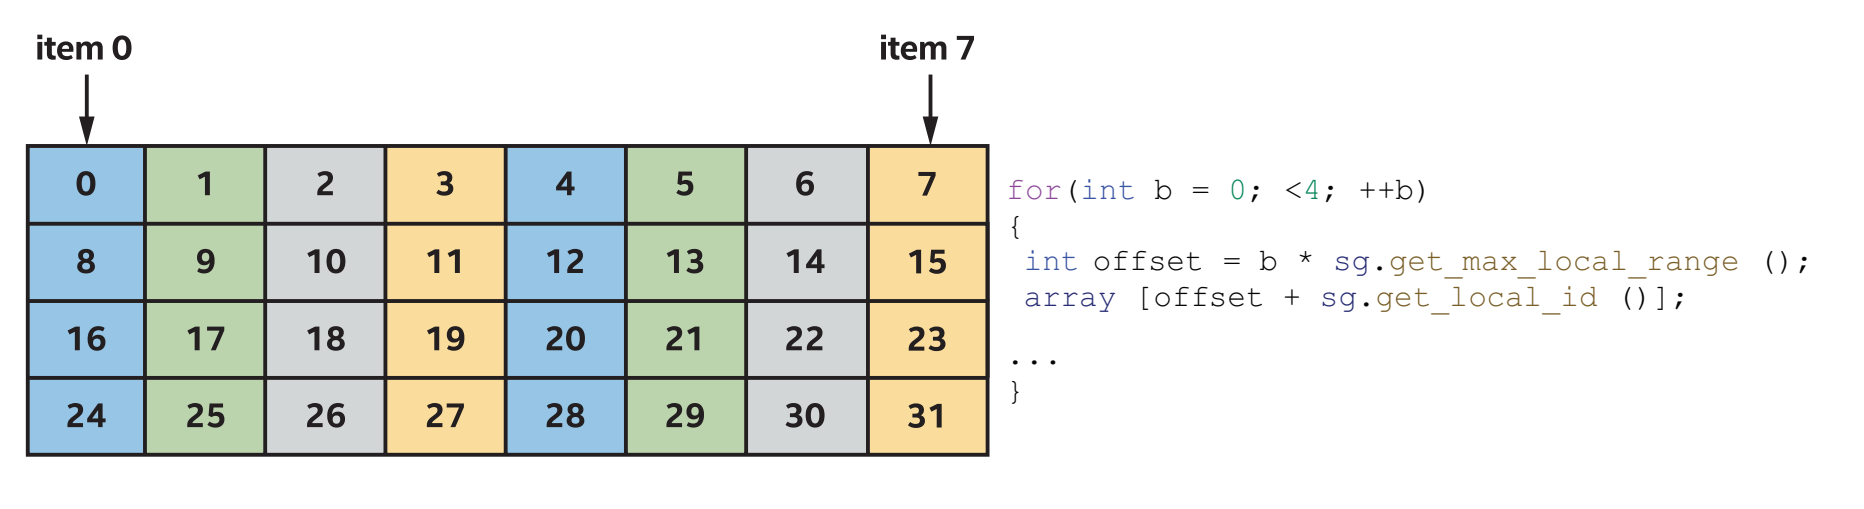
\includegraphics[width=1.\textwidth]{content/chapter-9/images/13}
\end{center}

Some architectures include dedicated hardware to detect when workitems in a sub-group access contiguous data and combine their memory requests, while other architectures require this to be known ahead of time and encoded in the load/store instruction. Sub-group loads and stores are not required for correctness on any platform, but may improve performance on some platforms and should therefore be considered as an optimization hint.\par

































